\chapter{Agilité et Scrum}

\section{Méthodes Agiles}

\subsection{Présentation}
Les méthodes de développement dites "méthodes agiles" (en anglais Agile Modeling) visent à réduire le cycle de vie du logiciel (donc accélérer son développement) en développant une version minimale, puis en intégrant les fonctionnalités par un processus itératif basé sur une écoute client et des tests tout au long du cycle de développement. 

L'origine des méthodes agiles est liée à l'instabilité de l'environnement technologique et au fait que le client est souvent dans l'incapacité de définir ses besoins de manière exhaustive dès le début du projet. Le terme "agile " fait ainsi référence à la capacité d'adaptation aux changements de contexte et aux modifications de spécifications intervenant pendant le processus de développement. 

\subsection{Principes et fonctionnement de la méthode Agile}

Le principe de base des méthodes "Agile" est qu’il est contre-productif de développer un produit, en planifiant et en spécifiant les moindres détails. 
En effet, prévoir tous les aspects de la production entraîne dans la plupart des cas frustrations et pertes de temps car les aléas surviennent fréquemment. C’est cette approche prédictive et séquentielle de type cascade ou cycle en V que les tenants des méthodes "Agile " veulent casser. Ainsi, au lieu de fixer les objectifs lointains, le mieux serait de procéder par étapes c’est-à-dire fixer des objectifs à court terme et commencer le développement sans perdre de temps. Chaque fois que cet objectif est atteint, on passe au prochain et ainsi de suite jusqu’à atteindre le but ultime. Au niveau d’un développement de logiciel, c’est le client qui transmet à l’équipe de développeurs sa vision du produit avec la liste des fonctionnalités qu’aurait ce produit. Il communique ainsi directement avec l’équipe et ensemble ils estiment le coût de chaque fonctionnalité pour aboutir à une idée approximative du budget final. De ce fait, on raisonne plus "produit" que "projet", d’où l’utilisation du terme "gestion de produit" au lieu de "gestion de projet".

\subsection{Valeurs fondamentales}
4 valeurs fondamentales provenant du manifeste Agile. 

\begin{enumerate}
\item \textbf{L'équipe} ("Les individus et leurs interactions, plus que les processus et les outils") : dans l'optique agile, l'équipe est bien plus importante que les outils (structurants ou de contrôle) ou les procédures de fonctionnement. Il est préférable d'avoir une équipe soudée et qui communique, composée de développeurs (éventuellement à niveaux variables), plutôt qu'une équipe composée d'experts fonctionnant chacun de manière isolée. La communication est une notion fondamentale.
\item \textbf{L'application} ("Des logiciels opérationnels, plus qu'une documentation exhaustive ") : il est vital que l'application fonctionne. Le reste, et notamment la documentation technique, est une aide précieuse mais non un but en soi. Une documentation précise est utile comme moyen de communication. La documentation représente une charge de travail importante, mais peut pourtant être néfaste si elle n'est pas à jour. Il est préférable de commenter abondamment le code lui-même, et surtout de transférer les compétences au sein de l'équipe (on en revient à l'importance de la communication).
\item \textbf{La collaboration} ("La collaboration avec les clients, plus que la négociation contractuelle ") : le client doit être impliqué dans le développement. On ne peut se contenter de négocier un contrat au début du projet, puis de négliger les demandes du client. Le client doit collaborer avec l'équipe et fournir un compte rendu continu sur l'adéquation du logiciel avec ses attentes.
\item \textbf{L'acceptation du changement} ("L'adaptation au changement, plus que le suivi d'un plan") : la planification initiale et la structure du logiciel doivent être flexibles afin de permettre l'évolution de la demande du client tout au long du projet. Les premières livraisons du logiciel vont souvent provoquer des demandes d'évolution.
\end{enumerate}

\subsection{Principes généraux}

Ces quatres valeurs se déclinent en 12 principes généraux communs à toutes les méthodes agiles. 
\begin{enumerate}
    \item  La plus haute priorité est de satisfaire le client en livrant rapidement et régulièrement des fonctionnalités à forte valeur ajoutée.
    \item Le changement est accepté, même tardivement dans le développement, car les processus agiles exploitent le changement comme avantage concurrentiel pour le client.
    \item La livraison concerne une application fonctionnelle, toutes les deux semaines à deux mois, avec une préférence pour la période la plus courte.
    \item Le métier et les développeurs doivent collaborer régulièrement et de préférence quotidiennement au projet.
    \item Le projet doit impliquer des personnes motivées. Donnez-leur l'environnement et le soutien dont elles ont besoin et faites leur confiance quant au respect des objectifs.
    \item La méthode la plus efficace pour transmettre l'information est une conversation en face à face.
    \item L’unité de mesure de la progression du projet est un logiciel fonctionnel (ce qui exclut de comptabiliser les fonctions non formellement achevées).
    \item Les processus agiles promeuvent un rythme de développement soutenable (afin d’éviter la non qualité découlant de la fatigue).
    \item Les processus agiles recommandent une attention continue à l'excellence technique et à la qualité de la conception.
    \item La simplicité et l'art de minimiser les tâches parasites, sont appliqués comme principes essentiels.
    \item Les équipes s'auto-organisent afin de faire émerger les meilleures architectures, spécifications et conceptions.
    \item À intervalle régulier, l'équipe réfléchit aux moyens de devenir plus efficace, puis accorde et ajuste son processus de travail en conséquence.
\end{enumerate}


\section{Scrum}

Scrum est un schéma d’organisation de développement de produits complexes. Il est défini par ses créateurs comme un "cadre de travail permettant de répondre à des problèmes complexes et changeants tout en livrant de manière productive et créative des produits de la plus grande valeur possible ". Scrum est considéré comme une méthode agile.
\jumpOne
La méthode s'appuie sur le découpage d'un projet en boîtes de temps, nommés "sprints ". Les sprints peuvent durer entre quelques heures et un mois (avec une préférence pour deux semaines). Chaque sprint commence par une estimation suivie d'une planification opérationnelle. Le sprint se termine par une démonstration de ce qui a été achevé. Avant de démarrer un nouveau sprint, l'équipe réalise une rétrospective. Cette technique analyse le déroulement du sprint achevé, afin d'améliorer ses pratiques. L'adaptation et la réactivité de l'équipe de développement est facilitée par son auto-organisation.


\subsection{Fonctionnement du Scrum}

\subsubsection{Piliers du scrum}

\begin{enumerate}
\item \textbf{La transparence} : Scrum met l'accent sur le fait d'avoir un langage commun entre l'équipe et le management. Ce langage commun doit permettre à tout observateur d'obtenir rapidement une bonne compréhension du projet.
\item \textbf{L'inspection }: À intervalle régulier, Scrum propose de faire le point sur les différents artéfacts produits, afin de détecter toute variation indésirable.

Ces inspections ne doivent pas être faites trop fréquemment, ou par un inspecteur mal formé : cela nuirait à l'avancement du projet.
\item \textbf{L'adaptation} : Si une dérive est constatée pendant l'inspection, le processus doit alors être adapté. Scrum fournit des rituels, durant lesquels cette adaptation est possible. Il s'agit de la réunion de planification de sprint, de la mêlée quotidienne, de la revue de sprint ainsi que de la rétrospective de sprint.
\end{enumerate}

\subsection{Caractéristiques}

Le framework Scrum consiste en la définition des rôles projets, activités ou artefacts, et réunions ou événements.

\subsubsection{Rôles}
Scrum définit trois rôles : \textit{Product Owner}, \textit{le Scrum Master} et le \textit{Développeur}. Il est à noter que le rôle de développeur couvre plusieurs métiers d'une organisation traditionnelle.

\begin{description}
    \item \textbf{Product Owner} est le représentant des clients et des utilisateurs. Il est "responsable de maximiser la valeur du produit et du travail de l'équipe de développement".  Il est seul à diriger l'activité de l'équipe de développement. 
    
    Par conséquent, cet acteur se charge de différents "sous-rôles" et à plusieurs responsabilités 
    \begin{itemize}
    \item Il explicite les éléments (Items) du Carnet du produit.
    \item C'est lui qui définit l'ordre dans lequel les fonctionnalités seront développées. Il prend les décisions importantes concernant l'orientation du projet.
    \item Il s'assure que le carnet du produit est visible et compris de l'équipe de développement.
    \end{itemize}
    
    C'est également lui qui, en accord avec l'équipe, fixe les objectifs d'un incrément (Sprint) au début de celui-ci. Si ces objectifs deviennent obsolètes pendant le sprint, il a alors la possibilité d'interrompre le sprint en cours.

Dans l'idéal, travaille dans la même pièce que l'équipe. Il est important qu'il reste très disponible pour répondre aux questions de l'équipe et pour lui donner son avis sur divers aspects du logiciel.

    \newpage
    
    \item \textbf{Scrum master} : Il aide le groupe à apprendre et à appliquer le Scrum afin que la valeur métier se
matérialise. Le ScrumMaster fait tout ce qui est en son pouvoir pour aider l’equipe, le product
owner et l’organisation à réussir le projet. Il n’est pas le manager de l’Equipe, ni
même un chef de projet, un chef d’équipe ou un représentant de l’equipe. Son rôle est plutôt de
servir l’equipe; il aide à supprimer les obstacles, protège les développeurs des interférences extérieures, et
facilite l’adoption par les développeurs des pratiques modernes du développement. 

Il enseigne, il coache et guide le Product Owner, les développeurs ainsi que le reste de l’organisation dans une utilisation fine de Scrum. Il s’assure que chacun (y compris le Product Owner, ainsi que le top management) comprenne les principes et les pratiques de Scrum, et il accompagne l’organisation dans le changement souvent difficile mais nécessaire au succès du développement agile. 

Etant donné que Scrum met en lumière les obstacles et les menaces qui pèsent sur l’efficacité des développeurs et du Product Owner, 
il est important d’avoir un Scrum Master engagé et travaillant énergiquement à la résolution des problèmes auxquels seront confrontés aussi bien l’équipe que le Product Owner. 
Il y a idéalement un ScrumMaster dédié et à plein temps, bien qu’une petite équipe puisse voir l’un de ses membres jouer ce rôle (on réduit alors sa charge sur les travaux courants).  
    \item \textbf{L'équipe de développement, les développeurs}. construit le produit qui est défini par le Product Owner : une application ou un site web par exemple. 

Dans Scrum, l’Equipe est "plurifonctionnelle" : elle inclut toute l’expertise nécessaire pour fournir une version du produit potentiellement livrable à chaque Sprint. 

Elle est également "auto organisée" (autogérée), avec un grand degré d’autonomie et de responsabilité. L’équipe décide des éléments à implémenter dans un Sprint (éléments issus de la liste proposée par le Product Owner), et des moyens les plus adaptés pour réaliser cet objectif.

Chaque personne dans l’Equipe est simplement qualifiée de membre. Il faut noter qu’il n’y a pas de
titre de spécialiste au sein d’un groupe qui adopte Scrum; pas d’analyste fonctionnel, pas de DBA,
pas d’architecte, pas de team leader, pas de concepteur IHM, pas de programmeur. 


Tous les membres travaillent ensemble durant chaque Sprint, par tous les moyens appropriés et 
nécessaires à l’atteinte de l’objectif qu’ils ont eux-mêmes déterminé.

Etant donné qu’il n’y a que des membres, l’Equipe n’est pas seulement pluridisciplinaire mais fait
également preuve de capacité diverse d’apprentissage; chacun possède certainement des atouts
particuliers, mais continue également de progresser sur d’autres spécialités. 

Chaque personne devra posséder des compétences sur différents domaines et à différents niveaux, et devra "aller là où le travail se trouve". Les individus doivent être à même de prendre en charge des tâches dans des
domaines moins familiers lorsqu’il est nécessaire de faciliter la finalisation d’un élément. 

 Dans Scrum, les Equipes sont plus productives et efficaces si tous les membres sont
dédiés à 100\% à un seul produit au cours d’un Sprint. Afin d’éviter des changements de contextes et
un fléchissement dans la focalisation, inconvénients souvent coûteux, il faut éviter la multiplication
des tâches entre plusieurs projets ou produits. Les équipes stables étant plus productives, il faut
éviter les changements au sein de l’équipe.

\end{description}

\newpage

\subsubsection{Scrum Master et Product Owner ne peuvent être la même personne}

Le scrum master et le product owner, ne peuvent pas être la même personne tant leurs objectifs sont différents et la combinaison des deux rôles conduits souvent à la de la congusion et des conflits. 
En effet cette combinaison va pousser le PO à faire du micro management, ce qui est à l'opposé des équipes auto-organisées telles que Scrum le définit. 
A la différence d'un manager classique, le scrum master ne dit pas à chacun ce qu'il doit faire et n'assigne pas de tâches. Il facilite le processus en soutenant les développeurs dans son organisation et sa gestion. Si le scrum master était précédemment en position de chef de projet au sein des développeurs, il devra changer significattivement d'état d'esprit pour que les développers puissent pleinement profiter du scrum. 

\subsubsection{Scrum sans chef de projet ?}

On pourra noter qu'il n'existe pas de chef de projet dans la méthologie scrum. En réalité il n'est pas nécessaire. 
Les responsabilités traditionnellement associées au chef de projet ont été divisées et réassignées aux trois rôles de scrum et principalement aux développeurs et au product owner, plutôt qu'au scrum master. 
Pratiquer le scrum en y ajoutant un chef de projet indique une méconnaissance fondamentale de scrum et conduit typiquement à des conflits dans les reponsabilités, un manque de clarté dans l'autorité et au final de piètres résultats. 
Parfois un ancien chef de projet peut jouer le rôle de scrum master, mais la réussite de cette approche est largement dépendante des individus et de la façon dont ils comprennent les différences fondamentales entre ces deux positions.

\subsubsection{Adaptation des autres acteurs du projet au Scrum}

En plus des trois rôles, d'autres parties prenantes contribuent au succès du projet. Parmi elles, les manager, clients et les utilisateurs. 
Certaines parties prenants, telles que les directions fonctionnelles ou techniques pourront voir évoluer significativement leurs rôles dans une organisation adoptant le Scrum, mais ils gardent néanmoins toute leur valeur. 

\begin{itemize}
    \item Ils soutiennent l'équipe en respectant les règles et l'esprit de scrum
    \item Ils aident à supprimer les obstacles que l'équipe et le product owner identifient
    \item Ils fournissent leur expertise et leur expérience. 
\end{itemize}

Ainsi ces personnes ne sont plus considérés comme des micro-manager (assignant des tâches, obtenant l'état d'avancement, etc) mais deviennent les véritables serviteurs de l'équipe de développement. 
Par le biais de conseils, coaching, facilitant la suppression des obstacles et la résolution des problèmes, fournissant des idées créatives, et apportant leurs compétences aux membres de l'équipe de développeurs.


\section{Artéfact du scrum}

\subsection{Product Backlog}

Lorsqu'une entreprise décide d'utiliser Scrum sur un projet, avant même de pouvoir démarrer le premier sprint elle a besoin d'un \textbf{product backlog} ou \textbf{carnet de produit}, correspondant à une liste priorisée (ordonnée) des caractéristiques orientées client. 

C'est l'unique source des besoins pour tous les changements à effectuer sur le produit. 
Le product backlog est un document qui évolue constamment au cours de la vie du produit et n'est jamais réellement terminé. 

Il n'existe qu'un seul product backlog pour un produit. 

\subsubsection{Contenu}

Ce carnet de produit, va contenir une variété d'élements : 

\begin{itemize}
\item \textbf{Nouvelles fonctionnalités métier}, possibilité pour chaque utilisateur d'ajouter un article au panier
\item \textbf{Objectifs majeurs d'ingénierie}, réécrire le système PHP en Java
\item \textbf{Améliorations technique}, refonte du module de transactions afin de le rendre plus extensible
\item \textbf{Travaux exploratoires}, étudier une solution de stockage plus rapide que celle actuelle
\item A\textbf{nomalie connu du système}\footnote{
Les anomalies sont dans le product backlog dans le cas ou elles sont peu nombreuses. }, diagnostiquer et corriger l'erreur dans le script de traitement des commandes. 
\end{itemize}


Tout ces éléments, sont élaborés de différentes manières à partir du moment ou ils restent clairs et viables sur la durée du projet. 


\begin{figure}[h!]
\centering
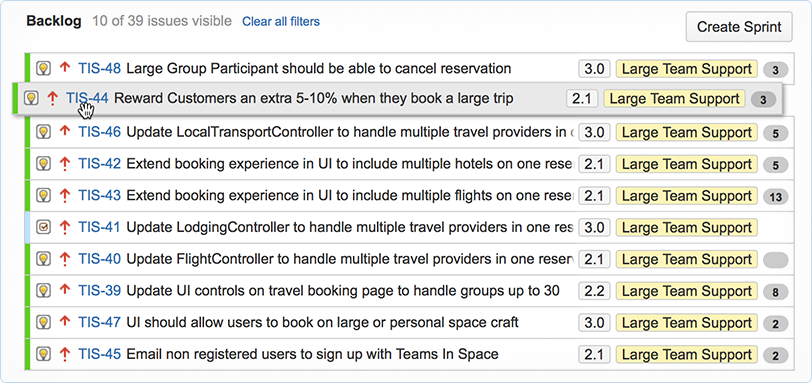
\includegraphics[width=1\textwidth]{assets/product_backlog.png}
\caption{Exemple d'un product backlog sur le logiciel JIRA, contenant plusieurs tâches}
\label{fig:my_label}
\end{figure}

Chaque élement du product backlog doit être : 

\begin{description}
    \item[Détaillé]{Les éléments les plus prioritaires sont de granularité plus fine et sont plus détaillés que les autres.}
    \item[Estimé]{Chaque élement doit être estimé au préalable et peut être réestimé à chaque sprint, en fonction des nouvelles informations apparues et de la connaissance acquise. A chaque début de sprint, l'équipe fournit au product owner, une estimation de l'effort requis pour chaque élément du product backlog et des risques techniques éventuels. }
    \item[Flexible]{Du fait de la nature du scrum, le product backlog est affiné régulièrement. Les élements peuvent être modifiés, ajoutés, supprimés à chaque sprint. Ainsi le Product Backlog est continuellement mis à jour par le product owner afin de refléter les évolutions du besoin client, les nouvelles idées ou enseignements, les mouvements de la concurrence, les obstacles techniques qui apparaissent, etc.}
    \item[Priorisé]{Les élements sont ordonnés par ordre de point d'effort. En général les élements plus prioritaires doivent être "rentable". Une plus grande valeur métier pour un moindre coût. L'augmentation de la priorité d'un élement peut également être motivée par la nécessité de s'attaquer aux risques importants, avant qu'ils n'apparaissent.}
\end{description}

L'estimation de élements permet d'avoir de manière approximative une projection dans le temps d'une potentielle date de release incluant une certain nombre de fonctionnalité. 



\subsection{Sprint backlog}

A chaque début de Sprint, un but est décidé. Pour atteindre cet object, l'équipe de développement choisit lors de la réunion de planification de sprint quels élements du product backlog seront réalisés. 

Ces élements sont alors groupés dans un carnet de sprint.
Ainsi chaque personne de l'équipe met à jour régulièrement le carnet de sprint au cours de son activité, afin que celui-ci donne une vision la plus précise possible de ce que l'épique prévoit de réaliser pour atteindre les objectifs du sprint. Le carnet de sprint est sous la responsabilité de l'équipe et elle seule peut la modifier en cours d'itération. 

\begin{figure}[h!]
\centering
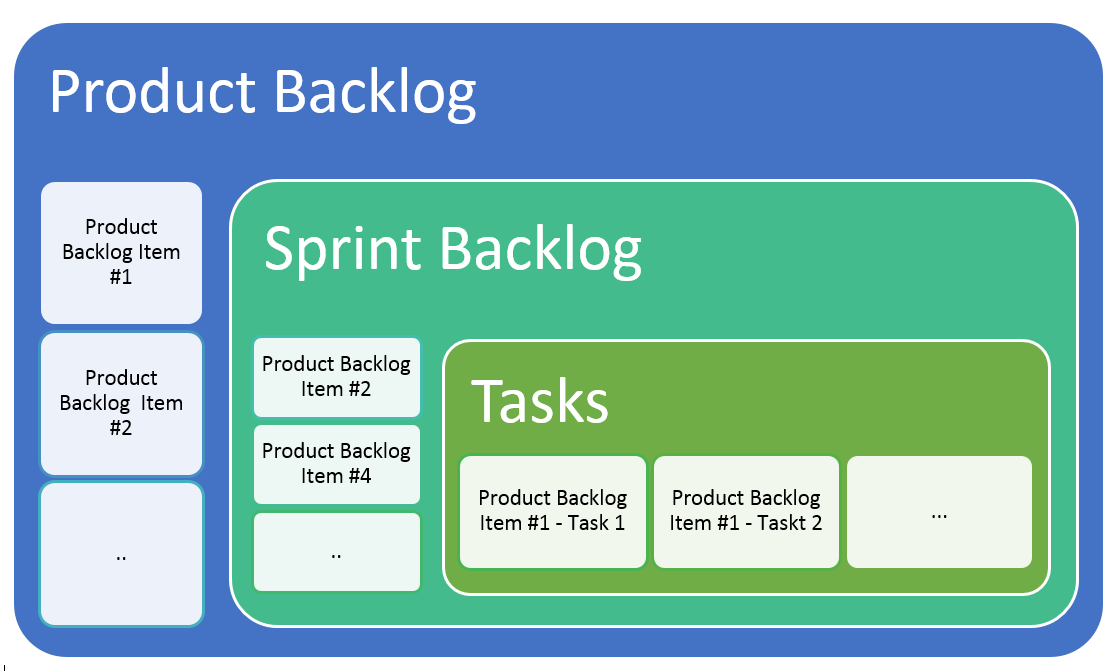
\includegraphics[width=0.7\textwidth]{assets/backlog.png}
\caption{Hiérarchie des backlog}
\label{fig:my_label}
\end{figure}


\subsection{Incrément de produit}

Chaque sprint, doit produire ce qui est officiellement appelé un incrément du produit, potentiellement livrable. 

C'est l'ensemble des des éléments du Sprint backlog finis pendant ce sprint et ceux pendant les sprint précédents. Les élements sont dits dans un état terminé lorsqu'ils remplissent leur rôle et qu'ils peuvent être utilisés directement. 

\section{Evénements}


\subsection{Sprint}
C'est l'évenement principal du scrum. C'est une période d'un mois maximum, durant laquelle l'équipe travaille et au bout duquel elle délivre un incrément du produit. 

La durée du Sprint est toujours la même durant tout le projet et un nouveau sprint démarre à chaque fois qu'un autre se termine. 



\begin{description}
    \item[Chaque sprint possède un but et sprint backlog]
    {
        Cependant, durant le sprint 
        
        \begin{itemize}
        \item l'objet ne peut être modifié
        \item la composition de l'équipe reste constante
        \item la qualité n'est pas négociable
        \item le sprint backlog est sujet à négociation entre le product owner et les développeurs. 
        \end{itemize}
    }
    \item[Limitation temporelle]
    {Un sprint peut durer au maximum un mois afin de limiter sa complexité et donc les risques liés au sprint. Chez Bob el web, la temps optimal est de 2 semaines
    }
    \item[Objet]
    {
        Si l'objet du sprint devient obsolète pendant celui-ci, le product owner peut décider de l'annuler en conséquence.  
        Ainsi les développements qui ont été terminés sont revus par le proriétaire du produit et peuvent être acceptés. 
        Ceux n'étant pas acceptés sont réestimés et remis dans le sprint backlog ce qui provoque le démarrage d'un nouveau sprint. 
    }
\end{description}



\subsection{Daily Scrum}

Dès que le sprint début, les développeurs se lancent quand une autre pratique fondamentale du scrum, le dail scrum (ou mêlée quotidienne en français). 
Il s'agit d'une courte réunion qui se déroule chaque jour de travail à heure fixe. Tout le monde y participe. 
Afin de garantirr que la réunion soit courte, il est nécessaire qu'elle se fasse en étant debout. 

C'est l'opportunité pour l'équipe de synchroniser ses travaux et d'échanger ensemble sur les obstacles recontrés ou à venir. 

Chaque membre de l'équipe expose successivement aux autres 3 points.

\begin{enumerate}
\item Qu'a-t-il fait depuis la dernière réunion ? 
\item Que va-t-il faire jusqu'à la prochaine réunion ? 
\item Quels sont les points d'obstacles ou de blocage rencontrés ou à prévoir ? 
\end{enumerate}


Il est important de noter que le daily scrum n'est pas une réunion de suivi pour le reporting à un manager. C'est au contraire le moment privilégié pour une équipe auto-organisé d'échanger sur la bonne marched l'activité et de se coordonner. 
En réalité pendant cette réunion, il n'y a presque pas de discussion et chacun doit juste répondre aux 3 questions. 
Si des discussions supplémentaires sont nécessaires, elles se tiennent lors de réunios consécutives, immédiatement après le daily scrum. 

Ces réunions sont un moyen supplémentaire d'inspection et d'adaptation. 


\subsection{Revue de Sprint}
Chaque fin de Sprint donne lieu à une revue de Sprint et une réunion de planification (préparant le prochain sprint). 

Cette réunion est prévue pour l'équipe et le product owner passent en revue le sprint qui vient de se terminer. 
Sont présents à cette réunion 

\begin{itemize}
\item L'équipe de développeurs
\item Le scrum master
\item Le product Owner
\item Les clients
\item Toute partie prenant, experts, décieurs et personnes intéressés. 
\end{itemize}

Chaque personne est libre de poser des questions ou d'apporter des contributions. 


L'objectif n'est pas réellement de faire une "démo" du travail accompli mais plutôt de regarder et d'étudier ce qu'il se passe et ainsi permettre de s'améliorer sur la base d'évaluations, en cycles itératifs. 
C'est également un excellent moyen pour le product owner de connaitre la situation actuelle du produit et de l'équipe de connaitre la situation actuelle du product owner du métier. 
Il est donc primordial qu'une conversation en profondeur s'établisse entre l'équipe et le product owner afin d'échanger sur la situation, obtenir des conseils, etc. 


\subsection{Réunion de préparation du prochain sprint}
A la suite de la revue de sprint, le product owner peut appliquer toute nouvelle mise à jour au product backlog. 
Il n'y a pas d'arrêt entre les sprints.

Par exemple, chez Bob el web les sprints durent 2 semaines, la revue de sprint s'effectue le vendredi matin et la préparation du prochain sprint le vendredi en début d'après midi après le daily scrum. 
\jumpOne
L'un des principes du développement agile est l'application d'un rythme soutenable, et c'est uniquement en travaillant aux heures normales et à une cadence raisonnable que les développeurs peuvent continuer ce cycle indéfiniment. 
La productivité des développeurs augment avec le temps grâce à l'évolution des pratiques et la suppression des obstacles qui ralentissent la cadence, et non pas en augmentant la charge de travail ou en faisant des compromis sur la qualité. 
\jumpTwo
Les sprints s'enchainent donc, jusqu'à ce que le product owner décide que le produit est prêt à être sorti. (Qu'une release sorte). 
Le summum du scrum, c'est qu'\textbf{un produit est potentiellement livrable à la fin de chaque sprint}, c'est à dire sans aucun travaux à terminer tels que des tests ou de la documentation.
Cela implique évidemment que tout soit complètement terminé à chaque Sprint, de telle sorte qu'il soit réellement possible de livrer le produit ou de le déployer immédiatement après la revue de sprint. 
\jumpOne
Cependant beaucoup d'organisations, possèdent des pratiques de développement, des outils et une infrastructure inadaptée et sont dans l'incapacité d'aboutir à cette vision de la perfection.
(On notera que les outils et l'infrastructure adapté est abordé dans la seconde partie de ce rapport). 


\begin{figure}[h!]
\centering
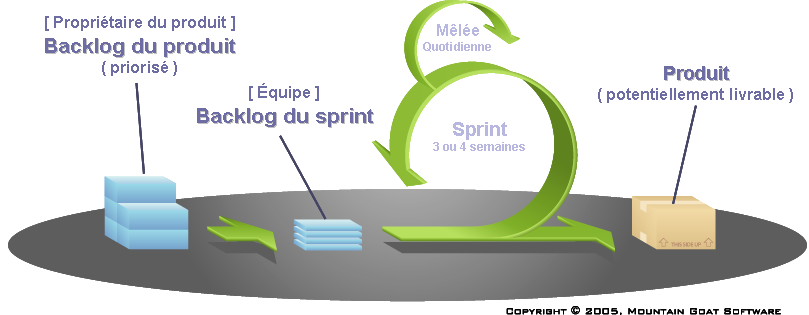
\includegraphics[width=0.8\textwidth]{assets/scrum.png}
\caption{Vue globale}
\label{fig:my_label}
\end{figure}

\newpage

\section{Développement de logiciel à travers la méthode agile chez Bob}
% Qu'est-ce qui était avant ? 
L'entreprise est passé d'une utilisation Agile light (avec seulement une liste de ticket à faire, au fur et a mesure) en Scrum il y'a plus d'un an. 

% Pourquoi Scrum ?
Le directeur technique de l'entreprise, Fred Wolf a pu aller voir le fonctionnement du scrum, par une équipe réelle par le biais d'un actionnaire. 
Le scrum est très adapté à Bob en raison du petit nombre de salariés.

% Av/In

D'un point de vue pratique et sur le terrain, le scrum permet chez Bob d'avoir une vision à moyen et court terme en se concentrant sur des tâches "éclatées", plutôt courtes et moyennement complexes. 

Cependant, le fait de changer souvent de tâches, voir de projet peut avoir des effets négatifs sur l'équipe de développeurs, qui doit constamment jongler entre plusieurs choses. 
Il est également plus difficile de donner des deadlines à long terme, puisqu'on avance par Sprint. 




% Montrer ici que le scrum était très intéressant 
% Depuis combien de temps êtes vous passés en mode Agile ?
%  on est passé en méthode Agile en mars 2014 (donc il y a un an et qq)
%- Vous utilisiez quoi avant ?
%avant on utilisait juste JIRA pour lister les tickets et on les faisait au fur et à mesure
%- Pourquoi avoir choisi l'agilité et le Scrum en particulier ?  Pour toi, quelles sont les avantages que l'agilité à apporter chez Bob?
%on a choisi Agile car cela nous permet de savoir où on va dans le temps tout en se concentrant sur des tâches relativement "atomiques" (donc plutôt courtes et moyennement complexes). Le Scrum en particulier je me souviens plus mais je crois qu'on a vite fait analyser les possibilités et c'était le plus approprié par rapport au nbre de personne chez BOB et à notre manière de travailler. En plus un de nos actionnaires gère une boîte qui fonctionne comme ça donc Fred a pu aller observer leur méthodologie avant de le mettre en place ici, mais on utilise de toute façon notre version du SCRUM qui n'est pas la version théorique mais une adaptation.
%- et les inconvénients ?
%les inconvénients sont le fait de changer souvent de tâche, voire de projet ce qui peut avoir des effets négatif (comme pour Fred quand il fait pas de PB pendant 3 semaines par exemple). et il est globalement plus difficile de donner des deadlines a moyen ou long terme pour les commerciaux.
